\begin{exercises} 
\item Suppose that $y = f(x)$ is a differentiable function for which the following information is known:  $f(2) = -3$, $f'(2) = 1.5$, $f''(2) = -0.25$.
\ba
	\item Is $f$ increasing or decreasing at $x = 2$?  Is $f$ concave up or concave down at $x = 2$?
	\item Do you expect $f(2.1)$ to be greater than $-3$, equal to $-3$, or less than $-3$?  Why?
	\item Do you expect $f'(2.1)$ to be greater than $1.5$, equal to $1.5$, or less than $1.5$?  Why?
	\item Sketch a graph of $y = f(x)$ near $(2,f(2))$ and include a graph of the tangent line.  
\ea
\begin{exerciseSolution}
\end{exerciseSolution}
\item For a certain function $y = g(x)$, its derivative is given by the function pictured in Figure~\ref{F:1.6.Ez2}.
\begin{figure}[ht]
\begin{center}
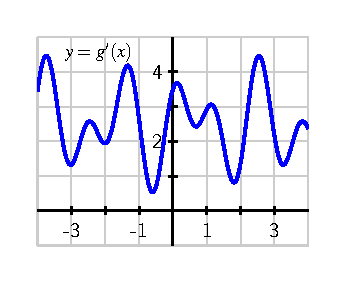
\includegraphics{figures/1_6_Ez2.eps}
\caption{The graph of $y = g'(x)$.} \label{F:1.6.Ez2}
\end{center}
\end{figure}
\ba
	\item What is the approximate slope of the tangent line to $y = g(x)$ at the point $(2,g(2))$?
	\item How many real number solutions can there be to the equation $g(x) = 0$?  Justify your conclusion fully and carefully by explaining what you know about how the graph of $g$ must behave based on the given graph of $g'$.
	\item On the interval $-3 < x < 3$, how many times does the concavity of $g$ change?  Why?
	\item Use the provided graph to estimate the value of $g''(2)$.
\ea
\item A bungee jumper's height $h$ (in feet ) at time $t$ (in seconds) is given in part by the data in the following table:

\begin{tabular}{ l | l | l | l |  l | l | l | l | l | l | l | l }
%\hline
$t$ & 0.0 & 0.5 & 1.0 & 1.5 & 2.0 & 2.5 & 3.0 & 3.5 & 4.0 & 4.5 & 5.0    \\ \hline %\hline 
\smallskip
$h(t)$ & 200 & 184.2 &  159.9 &  131.9 &  104.7 & 81.8 &  65.5 &  56.8 &  55.5 & 60.4 & 69.8 
\\ %\hline
\end{tabular}

\begin{tabular}{ l | l | l | l |  l | l | l | l | l | l | l  }
%\hline
$t$ & 5.5 & 6.0 & 6.5 & 7.0 & 7.5 & 8.0 & 8.5 & 9.0 & 9.5 & 10.0 \\ \hline %\hline
$h(t)$ & 81.6 & 93.7 &  104.4 &  112.6 &  117.7 & 119.4 & 118.2 & 114.8 &  110.0 &  104.7
\\ %\hline
\end{tabular}

\ba
	\item Use the given data to estimate $h'(4.5)$, $h'(5)$, and $h'(5.5)$.  At which of these times is the bungee jumper rising most rapidly?
	\item Use the given data and your work in (a) to estimate $h''(5)$.
	\item What physical property of the bungee jumper does the value of $h''(5)$ measure?  What are its units?
	\item Based on the data, on what approximate time intervals is the function $y = h(t)$ concave down?  What is happening to the velocity of the bungee jumper on these time intervals?
\ea

\item For each prompt that follows, sketch a possible graph of a function on the interval $-3 < x < 3$ that satisfies the stated properties.
\ba
	\item $y = f(x)$ such that $f$ is increasing on $-3 < x < 3$, $f$ is concave up on $-3 < x < 0$, and $f$ is concave down on $0 < x < 3$.
	\item $y = g(x)$ such that $g$ is increasing on $-3 < x < 3$, $g$ is concave down on $-3 < x < 0$, and $g$ is concave up on $0 < x < 3$.
	\item $y = h(x)$ such that $h$ is decreasing on $-3 < x < 3$, $h$ is concave up on $-3 < x < -1$, neither concave up nor concave down on $-1 < x < 1$, and $h$ is concave down on $1 < x < 3$.
	\item $y = p(x)$ such that $p$ is decreasing and concave down on $-3 < x < 0$ and $p$ is increasing and concave down on $0 < x < 3$.
\ea

\end{exercises}
\afterexercises